\documentclass[11pt,a4paper]{article}
\usepackage[no-math]{fontspec}
\usepackage{mathptmx}
\setmainfont{TeX Gyre Termes}
\usepackage{polyglossia}
\setdefaultlanguage[variant=british]{english}
\usepackage{amsmath,amssymb,bm}
\usepackage{booktabs,array,adjustbox}
\usepackage{graphicx}
\usepackage[labelfont=bf,labelsep=space,font=small,justification=centering]{caption}
\captionsetup[figure]{name=Fig.}\captionsetup[table]{name=Table}
\usepackage{lineno}
\usepackage[a4paper,margin=2.6cm]{geometry}
\usepackage{setspace}
\usepackage[authoryear,round]{natbib}
\bibpunct{(}{)}{;}{a}{}{,}
\usepackage{microtype}
\usepackage{enumitem}
\usepackage[hidelinks]{hyperref}
\usepackage{titlesec}
\usepackage[section]{placeins}
\titleformat{\section}{\normalfont\large\bfseries}{\thesection}{0.6em}{}
\titleformat{\subsection}{\normalfont\bfseries\itshape}{\thesubsection}{0.5em}{}
\titlespacing*{\section}{0pt}{2.2ex plus 1ex}{1.2ex}
\titlespacing*{\subsection}{0pt}{1.8ex plus 0.8ex}{0.8ex}
\setstretch{1.5}
\setlength{\parindent}{1.4em}
\setlength{\emergencystretch}{2em}
\renewcommand{\arraystretch}{1.08}
\setlist{nosep,leftmargin=1.6em}
\renewcommand{\floatpagefraction}{0.75}
\renewcommand{\topfraction}{0.85}
\renewcommand{\textfraction}{0.12}
\newcommand{\ipvaGrowth}{22.9}
\newcommand{\cpiGrowth}{23.5}
\newcommand{\realIpva}{$-$0.4}
\newcommand{\newGrowth}{19.3}
\newcommand{\existGrowth}{7.5}
\newcommand{\cpiTwoOne}{15.3}
\newcommand{\wNewtwotwo}{16.0}
\newcommand{\gNewtwotwo}{5.3}
\newcommand{\gExisttwotwo}{2.1}
\newcommand{\cNewtwotwo}{0.85}
\newcommand{\cExisttwotwo}{1.80}
\newcommand{\gTottwotwo}{2.7}
\newcommand{\cpiYtwotwo}{8.4}
\newcommand{\wNewtwothree}{14.6}
\newcommand{\gNewtwothree}{4.1}
\newcommand{\gExisttwothree}{2.4}
\newcommand{\cNewtwothree}{0.60}
\newcommand{\cExisttwothree}{2.03}
\newcommand{\gTottwothree}{2.6}
\newcommand{\cpiYtwothree}{3.5}
\newcommand{\wNewtwofour}{12.3}
\newcommand{\gNewtwofour}{8.8}
\newcommand{\gExisttwofour}{2.8}
\newcommand{\cNewtwofour}{1.08}
\newcommand{\cExisttwofour}{2.45}
\newcommand{\gTottwofour}{3.5}
\newcommand{\cpiYtwofour}{2.8}
\newcommand{\catNew}{53}
\newcommand{\catStock}{23}
\newcommand{\catN}{123}
\newcommand{\vsYear}{40}
\newcommand{\vsCcaa}{55}
\newcommand{\vsProv}{63}
\newcommand{\vsLdProv}{63}
\newcommand{\gSmall}{19.8}
\newcommand{\gBig}{25.0}
\newcommand{\bPop}{0.41}
\newcommand{\bPopSe}{0.16}
\newcommand{\bPopAR}{[0.03, 0.75]}
\newcommand{\bPopF}{17.9}
\newcommand{\bPopP}{1.08}
\newcommand{\bPopPAR}{[0.73, 1.46]}
\newcommand{\bViv}{$-$0.06}
\newcommand{\bVivAR}{[$-$0.50, 0.56]}
\newcommand{\bPre}{$-$0.02}
\newcommand{\bPreAR}{[$-$0.37, 0.43]}
\newcommand{\bPopUnwF}{5.2}
\newcommand{\bBig}{0.61}
\newcommand{\bBigAR}{[0.00, 2.46]}
\newcommand{\bSmall}{0.43}
\newcommand{\bSmallAR}{[$-\infty$, $\infty$]}
\newcommand{\bRentP}{0.38}
\newcommand{\bRentPAR}{[0.03, 0.75]}
\newcommand{\bInc}{0.39}
\newcommand{\bIncP}{0.07}
\newcommand{\tRCovid}{$-$0.30}
\newcommand{\tNCovid}{0.38}
\newcommand{\tRCovidP}{0.000}
\newcommand{\tNCovidP}{0.218}
\newcommand{\tRRecov}{0.44}
\newcommand{\tNRecov}{$-$0.96}
\newcommand{\tRRecovP}{0.001}
\newcommand{\tNRecovP}{0.011}
\newcommand{\tRLate}{0.28}
\newcommand{\tNLate}{0.23}
\newcommand{\tRLateP}{0.086}
\newcommand{\tNLateP}{0.663}
\newcommand{\tRPlacebo}{$-$0.14}
\newcommand{\tNPlacebo}{$-$0.26}
\newcommand{\tRPlaceboP}{0.316}
\newcommand{\tNPlaceboP}{0.503}
\newcommand{\ieetTwenty}{21}
\newcommand{\ieetTwentyOne}{60}
\newcommand{\ipvaEvTwelve}{$-$0.39}
\newcommand{\ipvaEvTwenty}{$-$0.20}
\newcommand{\ipvaEvTwentyFour}{$-$0.12}
\newcommand{\expMean}{1.4}
\newcommand{\expSd}{2.9}
\newcommand{\catExpMean}{1.3}
\newcommand{\catMunis}{274}
\newcommand{\vutTwenty}{321,496}
\newcommand{\vutTwentyFour}{403,267}
\newcommand{\vutTwentySix}{341,001}
\newcommand{\capROne}{$-$4.4}
\newcommand{\capNOne}{$-$18}
\newcommand{\capRdOne}{$-$3.7}
\newcommand{\capNdOne}{$-$19}
\newcommand{\capROneNever}{$-$5.0}
\newcommand{\capNOneNever}{$-$18}
\newcommand{\capRdOneNever}{$-$5.2}
\newcommand{\capNdOneNever}{$-$16}
\newcommand{\capRTwo}{$-$5.3}
\newcommand{\capNTwo}{$-$10}
\newcommand{\capRdTwo}{$-$6.7}
\newcommand{\capNdTwo}{$-$5}
\newcommand{\capGap}{6.1}
\newcommand{\provNew}{$-$0.57}
\newcommand{\provExist}{$-$0.19}
\newcommand{\catLeasesTwentyThree}{127,091}
\newcommand{\catLeasesTwentyFive}{102,272}
\newcommand{\cTotal}{20.6}
\newcommand{\cCpi}{21.1}
\newcommand{\cReal}{$-$0.4}
\newcommand{\cCap}{$-$5.9}
\newcommand{\cPop}{2.9}
\newcommand{\cPopLo}{0.2}
\newcommand{\cPopHi}{5.4}
\newcommand{\cPopM}{7.1}
\newcommand{\cPopTot}{1.9}
\newcommand{\cPopTotM}{4.9}
\newcommand{\cInc}{1.0}
\newcommand{\cIncLo}{$-$0.1}
\newcommand{\cIncHi}{2.2}
\newcommand{\incEl}{0.08}
\newcommand{\incReal}{13.5}
\newcommand{\cTourA}{0.16}
\newcommand{\cTourB}{$-$0.14}
\newcommand{\tourPerPpA}{0.13}
\newcommand{\dlnviv}{3.8}
\newcommand{\shPop}{12}
\newcommand{\catNewTwoFive}{19.0}
\newcommand{\capShare}{91}
\newcommand{\szAInfl}{5.4}
\newcommand{\szAVut}{1.5}
\newcommand{\szAPop}{2.2}
\newcommand{\szAR}{17.9}
\newcommand{\szAVutNinety}{4.6}
\newcommand{\szBInfl}{6.4}
\newcommand{\szBVut}{1.6}
\newcommand{\szBPop}{2.6}
\newcommand{\szBR}{19.6}
\newcommand{\szBVutNinety}{4.6}
\newcommand{\szCInfl}{6.3}
\newcommand{\szCVut}{1.2}
\newcommand{\szCPop}{2.6}
\newcommand{\szCR}{20.1}
\newcommand{\szCVutNinety}{3.8}
\newcommand{\szDInfl}{6.1}
\newcommand{\szDVut}{0.7}
\newcommand{\szDPop}{2.5}
\newcommand{\szDR}{19.7}
\newcommand{\szDVutNinety}{1.2}
\newcommand{\szEInfl}{10.8}
\newcommand{\szEVut}{1.4}
\newcommand{\szEPop}{4.4}
\newcommand{\szER}{22.2}
\newcommand{\szEVutNinety}{2.2}
\newcommand{\fjB}{0.07}
\newcommand{\fjLo}{$-$1.3}
\newcommand{\fjHi}{1.4}
\newcommand{\provPopB}{0.58}
\newcommand{\fjShare}{35}
\newcommand{\corpB}{0.028}
\newcommand{\corpLo}{$-$0.059}
\newcommand{\corpHi}{0.115}
\newcommand{\corpShare}{23}
\newcommand{\hutTotal}{104,548}
\newcommand{\hutPcB}{0.23}
\newcommand{\eurTwentyOne}{$-$0.49}
\newcommand{\eurTwentyThree}{3.87}
\newcommand{\mrTwentyOne}{1.92}
\newcommand{\mrTwentyThree}{3.13}


\title{\bfseries What Drives Rents in Spain? Demand, Supply, Tourism and Regulation across Municipalities}
\author{Víctor M. Fernández-Aguilera\\[4pt]
{\small University of Almería, Almería, Spain}\\
{\small Corresponding author. E-mail: vfa084@ual.es}}
\date{}

\begin{document}
\maketitle

\begin{abstract}\noindent
The rise of rents is one of Spain's main economic and political concerns, but the official index of rents on all leases in force grew by \ipvaGrowth\,\% between 2015 and 2024, as much as consumer prices. This paper asks which forces raised rents, in what order of importance, and where. A stock-flow model of the local rental market organises the candidate determinants and maps market rents into an index of all leases. Using tax-based rent indices for about 700 municipalities, the Catalan register of new leases, the INE count of tourist dwellings and four research designs, the paper finds, first, that the rise is a phenomenon of new contracts: in Catalonia, rents on new leases rose by \catNew\,\% between 2015 and 2024, against \catStock\,\% for all leases. Second, \vsLdProv\,\% of the variation in municipal rent growth is common within provinces, and cannot be attributed to local factors. Third, among local factors, population growth driven by immigration is the largest identified driver: a cumulative inflow of 1\,\% of the population raises the index by \bPop\,\%, and the housing stock does not respond. Fourth, tourist dwellings reallocate housing away from residents: when tourism collapsed in 2020--21, rents on new leases fell and more leases were signed where tourist dwellings were common, and the pattern reversed with the recovery; the effect is small on average and concentrated in tourist municipalities. Fifth, caps lowered measured rents: the 2024 Catalan cap reduced new-lease rents by about 5\,\%, and in its first wave the number of new leases fell by about 18\,\%. Associations with proxies for large owners are absent, and the roles of interest rates and credit are not identified.

\medskip\noindent\textbf{Keywords} Housing rents $\cdot$ Immigration $\cdot$ Tourist dwellings $\cdot$ Rent control $\cdot$ Housing supply $\cdot$ Spain\\
\textbf{JEL Classification} R21 $\cdot$ R31 $\cdot$ R38 $\cdot$ J61 $\cdot$ Z30
\end{abstract}
\clearpage
\linenumbers

\section{Introduction}\label{sec:intro}

Rents are at the centre of Spanish economic policy. Since 2019 governments have lengthened the minimum duration of leases, capped annual updates, allowed regions to cap rents in tensioned markets and restricted tourist dwellings, while public debate attributes the rise in rents to immigration, tourism, investment funds, interest rates or the lack of construction. Yet the official index of rents on all leases in force, the INE IPVA, rose by \ipvaGrowth\,\% between 2015 and 2024, while consumer prices rose by \cpiGrowth\,\%: measured in real terms, the average rent paid by Spanish tenants did not increase. This paper asks three questions. Which forces raised rents? In what order of importance? And where, by size of municipality and exposure to tourism, did each of them matter?

Answering them requires three things that are rarely combined. The first is a framework that says how each determinant should affect rents and what an index of all leases measures. Section~\ref{sec:theory} sets out a stock-flow model of the local market for long-term rentals in which population, income, tourist demand, supply, the user cost of owning and regulation enter through a single equilibrium condition. The model delivers five predictions and an identity linking market rents to the index of all leases: because only a small share of leases is renewed each year and the rest are indexed to inflation, the index of all leases moves slowly and follows inflation.

The second is a design for each determinant. Section~\ref{sec:data} combines tax-based rent indices for about 700 municipalities (2011--2024), the register of new-lease deposits in Catalonia by municipality and quarter (2019--2025), the INE count of tourist dwellings by municipality (2020--2026), cadastral dwelling counts, household income from the INE income atlas and population registers by country of birth. Population growth is instrumented with a shift-share prediction of immigrant arrivals; the effect of tourist dwellings is identified from the collapse of tourism in 2020--21 and the recovery that followed; the Catalan tensioned-zone cap is evaluated with stacked difference-in-differences; and the cap on annual updates is quantified with the accounting identity of the index.

The third is a clear separation between what the designs identify and what they do not. Designs that compare municipalities absorb shocks that are common to all of them, such as interest rates, national legislation and inflation. Ownership by large investors cannot be measured by municipality with public data. The paper therefore ranks determinants at three levels: the growth of the national index of all leases, the differences in rent growth across municipalities within provinces, and the growth of rents on new leases where they are observed.

The results are as follows. First, the rise in rents is concentrated in new contracts. Between 2021 and 2024, the INE index for new leases rose by \newGrowth\,\%, against \existGrowth\,\% for existing leases and \cpiTwoOne\,\% for consumer prices; in Catalonia, rents on new leases rose by \catNew\,\% between 2015 and 2024, against \catStock\,\% for all leases in the same municipalities (figure~\ref{fig:index}). Second, most of the variation in municipal rent growth is shared within provinces: province fixed effects account for \vsLdProv\,\% of the variance of growth between 2015 and 2024, and the year alone for \vsYear\,\% of the variance of annual growth. Third, the largest identified local driver is population growth driven by immigration: a cumulative foreign-born inflow equal to 1\,\% of the population raised the index of all leases by \bPop\,\% (Anderson-Rubin set \bPopAR), with no pre-trend and no response of the housing stock. Applied to the average inflow, it accounts for \cPop{} log points of the index's growth (range \cPopLo{} to \cPopHi). Fourth, tourist dwellings reallocate housing from residents to visitors: when tourism collapsed in 2020--21, rents on new leases fell by \tRCovid\,\% per percentage point of dwellings in tourist use relative to 2019, and the number of leases signed rose; with the recovery, rents rose by \tRRecov\,\% per point and the number of leases fell. Because tourist dwellings are a small share of the stock in most municipalities, this channel adds little to the national index but matters in tourist municipalities. Fifth, caps lowered measured rents. The cap on updates of existing leases held the index of all leases up to \capGap\,\% below the level it would have reached had leases followed consumer prices in 2022--2023. The Catalan tensioned-zone cap reduced rents on new leases by about 5\,\%, and in the first wave the number of new leases fell by about 18\,\%.

The paper contributes to three literatures. It adds to the work on the determinants of rents and house prices by estimating several channels within one framework and for a whole country, rather than one channel in one city \citep{saiz2007,garcialopez2020,barron2021}. It contributes to the measurement of rents by showing, with the index identity and new-lease data, that an index of all leases is a lagged and policy-distorted measure of market rents \citep{genesove2003,ambrose2015}. And it adds to the evaluation of Spanish housing policy, extending the evidence on the Catalan caps to 2025 and quantifying the cap on updates \citep{jofre2023,perez2026}. It builds on a companion paper on immigration and housing occupancy \citep{fernandez2026}, from which it takes the population instrument.

Section~\ref{sec:institutions} describes the institutional setting and the measurement of rents. Sections~\ref{sec:lit} and~\ref{sec:theory} review the literature and set out the framework. Section~\ref{sec:data} describes the data, section~\ref{sec:facts} the facts, and section~\ref{sec:determinants} the estimates for each determinant. Section~\ref{sec:ranking} ranks them, section~\ref{sec:discussion} discusses what the evidence does and does not support, and section~\ref{sec:conclusion} concludes.

\section{Institutional setting and measurement}\label{sec:institutions}

\textit{Leases.} Residential leases are governed by the 1994 Urban Leases Act. Royal Decree-law 7/2019, in force since 6 March 2019, extended the minimum duration of leases to five years when the landlord is a natural person and seven years when it is a company, and annual updates are typically tied to the consumer price index. Royal Decree-law 6/2022 of 29 March 2022 limited annual updates of existing leases to 2\,\%, a limit later extended to the end of 2023; the Housing Act (Law 12/2023 of 24 May) set a 3\,\% limit for 2024 and replaced the consumer price index with a new INE reference index from 2025. In the framework of section~\ref{sec:theory}, these measures act on the update rule $u_t$ and on the share of leases renewed each year, $\lambda_t$.

\textit{Rent caps in tensioned markets.} The Housing Act allows regions to declare tensioned residential markets, where rents on new leases are capped with reference to the rent of the previous lease and to a reference price index. Catalonia was the first region to apply it: 140 municipalities from 16 March 2024 and a further 131 from October 2024. A previous Catalan law (11/2020) had capped rents in 60 municipalities between September 2020 and March 2022, when the Constitutional Court annulled most of it \citep{jofre2023}.

\textit{Tourist dwellings.} Regions and municipalities regulate tourist dwellings through registers and licences. The INE experimental statistic counts dwellings advertised on the main platforms by municipality since August 2020; there were \vutTwenty{} in August 2020, \vutTwentyFour{} in August 2024 and \vutTwentySix{} in May 2026.

\textit{Measuring rents.} The IPVA is computed by INE from rents declared in personal income-tax returns. It covers all leases in force, not only new ones, and excludes the Basque Country and Navarre, which have their own tax administrations. It is published for municipalities with more than 10,000 inhabitants, with base 2015. Since 2021, INE also publishes separate indices for new and existing leases with their weights: new leases accounted for \wNewtwotwo\,\% of the index in 2022 and \wNewtwofour\,\% in 2024. Rents on new leases are observed by municipality only in Catalonia, where landlords must deposit the tenant's guarantee with the regional housing agency.

\section{What the literature says about each determinant}\label{sec:lit}

\textit{Population and immigration.} In spatial equilibrium, local rents capitalise the demand of residents who choose where to live \citep{roback1982}. Immigrant inflows provide a source of local demand shocks that can be predicted from earlier settlement patterns. With that strategy, \citet{saiz2007} estimates that an inflow equal to 1\,\% of a US metropolitan area's population raises rents by about 1\,\%, and \citet{sa2015} finds negative effects on house prices in England, explained by the out-migration of higher-income natives. For Spain, \citet{gonzalez2013} relate the immigration boom of 2000--2010 to house prices and construction, and \citet{sanchis2023} decomposes the price response by location. Shift-share instruments of this kind rely either on exogenous shares or on many exogenous shocks \citep{goldsmith2020,borusyak2022,adao2019}, and they can confound short- and long-run responses when settlement patterns are persistent.

\textit{Income, credit and the user cost.} Rents also capitalise local incomes and amenities \citep{roback1982,gyourko2013}, and the choice between renting and owning depends on the user cost of owner-occupation, which moves with interest rates, credit standards and expected price growth \citep{poterba1984,himmelberg2005,sinai2005}. These forces are largely common to all municipalities in a country, which is why the cross-sectional literature on local rents seldom identifies them. For Spain, \citet{khametshin2024} document that the rise in rental demand since 2015 is concentrated among young and foreign-born households and in large urban and tourist areas, and attribute part of it to prudent mortgage lending; they explicitly describe the quantification of each factor as an open question.

\textit{Supply.} Where supply is inelastic, demand shocks are capitalised into prices rather than accommodated by construction. Inelasticity reflects geography \citep{saiz2010} and regulation \citep{glaeser2018,hilber2016,molloy2020}, and housing durability makes supply asymmetric \citep{glaeser2005}. Constraints in productive cities have aggregate costs \citep{hsieh2019}. \citet{khametshin2024} show that rents grew more in large Spanish municipalities with less land available for building.

\textit{Tourist dwellings.} Home-sharing platforms raise long-term rents by moving dwellings from residents to visitors. \citet{barron2021} formalise this reallocation and estimate it with a shift-share instrument for the US; \citet{garcialopez2020} find that in Barcelona neighbourhoods with high Airbnb activity rents rose by several percentage points; \citet{koster2021} use regulatory borders in Los Angeles; and \citet{franco2021} and \citet{duso2024} report evidence for Portugal and Berlin. \citet{batalha2022} exploit the collapse of tourism in 2020 in Lisbon, which pushed short-term-rental dwellings back into the residential market and lowered rents. \citet{chaves2026} finds that Airbnb raised house prices and reduced residential inflows in Madrid neighbourhoods, and \citet{almagro2025} show how tourism reshapes neighbourhood amenities and sorting. Regulation of short-term rentals has its own effects \citep{valentin2021}.

\textit{Rent regulation.} Rent control lowers rents in covered units but reduces the supply of rental housing and can raise rents in uncovered segments \citep{autor2014,diamond2019}; \citet{kholodilin2024} reviews the evidence. In Catalonia, the 2020--2022 rent-containment law reduced rents and the number of leases signed \citep{jofre2023,monras2023}, and a first evaluation of the 2024 tensioned-zone cap finds a reduction in the number of new leases and a less robust effect on rent growth \citep{perez2026}.

\textit{Institutional investors.} In the United States, large buy-to-rent investors bought foreclosed single-family homes after 2008 \citep{mills2019}; the evidence on their effect on rents is mixed, with higher rents and fees in some markets \citep{gurun2023} and price stabilisation in others \citep{garriga2023}. In Spain, sociological and geographical work has documented the acquisition of rental portfolios by global funds and their role in tourist rentals \citep{janoschka2020,cocola2025}, but there is no causal estimate of their effect on rents. According to tax data compiled by \citet{khametshin2024}, companies owned 8.1\,\% of the dwellings let as main residences in 2021, ranging from 2.6\,\% to 11.1\,\% across regions.

\textit{Contribution of this paper.} Existing work studies one determinant at a time, usually in one city. This paper estimates several channels within a common framework, for all Spanish municipalities with an official rent index, distinguishes the stock of leases from new contracts, and states for each channel what the design identifies.


\section{A framework for the determinants of local rents}\label{sec:theory}

This section sets out a stock-flow model of a local market for long-term residential rentals. It serves three purposes: it organises the candidate determinants into a small number of channels, it states which of them can be identified from differences across municipalities and which only move all municipalities together, and it maps market rents into the rent index that is observed. The model follows the asset-and-space framework of \citet{dipasquale1992}, the user-cost approach to tenure choice of \citet{poterba1984}, and the landlord's choice between long- and short-term letting of \citet{barron2021}.

\subsection{Uses of the housing stock}

Municipality $i$ has a stock of $H_{it}$ dwellings in year $t$. Each dwelling is owner-occupied, let to a resident household on a long-term lease ($L$), let to visitors as a tourist dwelling ($S$), or kept out of the residential market as a second home or vacant unit ($V$). Construction changes $H_{it}$ slowly; in the short run the relevant margin is the allocation of the existing stock across uses.

\textit{Demand for long-term rentals.} Let $N_{it}$ be the resident population and $\theta_{it}$ the share of it that rents. The share renting falls with the rent relative to the user cost of owner-occupation, $\theta_{it}=\theta(R_{it}/U_t)$, where $U_t$ summarises mortgage rates, credit standards and expected price growth \citep{poterba1984,himmelberg2005}. Each renter consumes $q_{it}=A\,Y_{it}^{\alpha}R_{it}^{-\eta}$ dwellings per person, where $Y_{it}$ is income and $\eta\ge0$ is the price elasticity of space per person: a high $\eta$ means that households absorb higher rents by sharing dwellings or living at higher density rather than by paying more for the same space. Demand in dwelling units is $D_{it}=\theta_{it}N_{it}q_{it}$, so that
\begin{equation}\label{eq:demand}
d\ln D_{it}= d\ln N_{it}+\alpha\, d\ln Y_{it}+\varepsilon_\theta\, d\ln U_t-(\eta+\varepsilon_\theta)\,d\ln R_{it},
\end{equation}
with $\varepsilon_\theta=-\partial\ln\theta/\partial\ln(R/U)>0$.

\textit{Supply of long-term rentals.} An owner who lets a dwelling chooses the long-term market if the rent $R_{it}$ exceeds the expected net revenue from tourist letting, $P^S_{it}-c_j$, where $P^S_{it}$ is tourist revenue per dwelling and $c_j$ is an owner-specific cost of operating a tourist let (management, regulation, risk), distributed with cdf $G$. The share of lettable dwellings in tourist use is $s_{it}=G(P^S_{it}-R_{it})$. Owners also move dwellings between the rental market, owner-occupation and non-use as relative returns change, and the stock grows with rents in the long run with elasticity $\sigma_i$, which is low where land is scarce or development is restricted \citep{saiz2010,glaeser2018,hilber2016}. Writing $\varepsilon_\ell$ for the elasticity of the long-term rental share with respect to the rent, long-term supply satisfies
\begin{equation}\label{eq:supply}
d\ln L_{it}=(\sigma_i+\varepsilon_{\ell})\,d\ln R_{it}-\psi_{i}\,d\ln P^S_{it}+d\ln \tilde H_{it},
\end{equation}
where $\psi_i=\frac{s_i}{1-s_i}\,e_s$ is the elasticity of long-term supply with respect to tourist revenue, $e_s$ the elasticity of the tourist share with respect to $P^S$, and $d\ln\tilde H_{it}$ captures changes in the stock that are predetermined with respect to current rents.

\textit{Regulation.} A cap $\bar R_{it}$ on new-contract rents makes the long-term return $\min(R_{it},\bar R_{it})$. Where the cap binds, it lowers the rent on new contracts and moves owners at the margin to tourist or seasonal letting, sale or non-use: it reduces $L_{it}$ at a given market-clearing rent \citep{autor2014,diamond2019,jofre2023}.

\subsection{Equilibrium and predictions}

Equating \eqref{eq:demand} and \eqref{eq:supply},
\begin{equation}\label{eq:equilibrium}
d\ln R_{it}=\frac{1}{\Psi_i}\Big[\underbrace{d\ln N_{it}}_{\text{population}}+\underbrace{\alpha\,d\ln Y_{it}}_{\text{income}}+\underbrace{\psi_i\,d\ln P^S_{it}}_{\text{tourist demand}}-\underbrace{d\ln\tilde H_{it}}_{\text{supply}}+\underbrace{\varepsilon_\theta\,d\ln U_t}_{\text{user cost}}\Big],\qquad \Psi_i=\eta+\varepsilon_\theta+\varepsilon_\ell+\sigma_i .
\end{equation}
Equation \eqref{eq:equilibrium} delivers five predictions that structure the empirical analysis.

\begin{description}
\item[P1 (amplification).] A given demand shock raises rents more where $\Psi_i$ is small: where new supply is inelastic ($\sigma_i$ low), where few dwellings can be reallocated to long-term letting ($\varepsilon_\ell$ low), and where households cannot or do not absorb higher rents by sharing ($\eta$ low). Large, dense and land-constrained municipalities should show larger elasticities than small ones.
\item[P2 (tourist diversion).] Tourist demand affects long-term rents only through $\psi_i$, which is zero where there is no tourist-letting market and rises with the share of the stock in tourist use. The effect is symmetric: a collapse in tourist demand should lower long-term rents and raise the number of new long-term contracts most where tourist dwellings were most prevalent.
\item[P3 (rent caps).] A binding cap on new-contract rents lowers measured new-contract rents in covered municipalities and reduces the number of new long-term contracts, with larger effects in the upper part of the rent distribution, where the cap binds.
\item[P4 (common shocks).] The user cost of owning, credit standards, national legislation and inflation enter through $d\ln U_t$ and through terms common to all municipalities. Designs that compare municipalities within a year absorb them. Their contribution to national rent growth can only be assessed from national time series, without cross-sectional identification.
\item[P5 (ownership).] The identity of landlords enters the framework only through the distribution of costs $c_j$ (professional operators may face lower costs of tourist letting, raising $\psi_i$) or through market power, which requires a degree of local concentration. Without data on ownership by municipality the framework does not deliver a testable prediction for the effect of large investors on long-term rents.
\end{description}

\subsection{From market rents to the observed index}

The rent index used in this paper, the INE IPVA, is computed from rents declared in personal income-tax returns and covers all leases in force, not only new ones. Suppose that each year a share $\lambda_{it}$ of leases is new and signed at the market rent $R_{it}$, while existing leases are updated by a rule $u_t$ (the consumer price index, or a legal cap). The log of the average rent across leases then evolves approximately as
\begin{equation}\label{eq:index}
\Delta\ln\bar R_{it}\approx\lambda_{it}\big(\ln R_{it}-\ln\bar R_{i,t-1}\big)+(1-\lambda_{it})\,u_t .
\end{equation}
Equation \eqref{eq:index} has three implications. First, the stock index responds to market rents with a lag, so short-run elasticities estimated on it understate the response of new-contract rents by a factor of the order of $\lambda$ \citep{genesove2003,ambrose2015}. Second, a cap on the annual update of existing leases, such as the 2\,\% limit of 2022--2023, lowers the growth of the stock index even if market rents do not change. Third, a policy that regulates only new contracts is best evaluated with data on new contracts; this is why section~\ref{sec:regulation} uses the Catalan register of rental deposits, which records new contracts only.


\section{Data}\label{sec:data}

\textit{Rents.} INE IPVA by municipality (table 59060; 718 municipalities, 2011--2024), by province and type of contract (table 59005, 2021--2024) and nationally with the weights of new and existing leases (tables 59004 and 59008). In Catalonia, new leases signed and their average rent by municipality and quarter, from the deposit register published on the Generalitat's open-data portal (quarterly since 2019, annual before).

\textit{Population and the instrument.} Municipal register (2003--2022) and annual census (2021--2025) by country of birth. The foreign-born net inflow and its shift-share prediction are those of the companion paper: 33 origin groups, 2003 settlement shares and national growth excluding the own province, for 699 municipalities.

\textit{Tourism.} INE experimental statistic of tourist dwellings by municipality, August 2020 to May 2026 (tables 39363 and 39366), measured as a share of all dwellings. In Catalonia, the register of tourist establishments (104,548 active tourist dwellings, identifying whether the owner is a company) and the tourist-stay tax paid by tourist dwellings by municipality and semester, from 2017.

\textit{Supply, income and other inputs.} Cadastral dwellings by municipality (2013--2025), compiled from the Cadastre in the companion paper's replication package; net income per person from the INE household income atlas (2015--2023); foreclosures on dwellings by province and type of owner (INE, 2014--2025); the 12-month Euribor (ECB) and the average rate on new mortgages (INE); consumer prices (INE); and the Catalan designation of tensioned residential markets. Every file is downloaded by the replication code from the public source.

\section{What rose: new leases, cities and common shocks}\label{sec:facts}

Figure~\ref{fig:index} contrasts three measures. Nationally, the index of all leases fell until 2014, grew faster than consumer prices until 2021 and was overtaken by them in 2022--2024; over 2015--2024 the real change is \realIpva\,\%. The index for new leases, available from 2021, rose by \newGrowth\,\% to 2024, against \existGrowth\,\% for existing leases. In Catalonia, where new-lease rents are observed by municipality for a long period, they rose by \catNew\,\% between 2015 and 2024, more than twice the growth of the index of all leases in the same municipalities.

\begin{figure}[!htbp]\centering
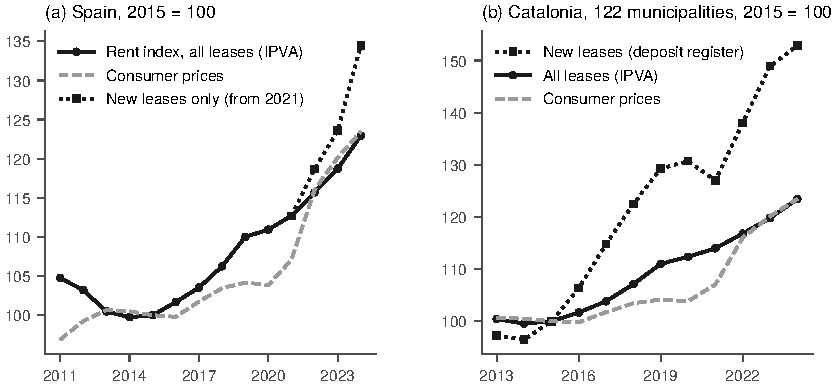
\includegraphics[width=\linewidth]{fig/fig1_index.pdf}
\caption{Rents on all leases, rents on new leases and consumer prices}\label{fig:index}
\begin{minipage}{0.95\linewidth}\footnotesize\vspace{2pt}
\textit{Notes}: panel (a), INE IPVA for all leases and for new leases (the latter chained to the former in 2021), and the consumer price index (annual averages). Panel (b), Catalan municipalities with both series in every year 2013--2024: average rent of new leases deposited with the regional housing agency and IPVA, means weighted by 2015 population. Sources: INE, Generalitat de Catalunya.
\end{minipage}
\end{figure}

The identity \eqref{eq:index} accounts for the gap. In 2024, new leases grew by \gNewtwofour\,\% and existing leases by \gExisttwofour\,\%; with a weight of \wNewtwofour\,\%, new leases contributed \cNewtwofour{} percentage points of the \gTottwofour\,\% growth of the index, and existing leases \cExisttwofour. In 2022, existing leases grew by \gExisttwotwo\,\% while consumer prices rose by \cpiYtwotwo\,\%: the cap on updates was binding. The weight of new leases fell from \wNewtwotwo\,\% in 2022 to \wNewtwofour\,\% in 2024, so that the index of all leases became even less sensitive to market rents.

Table~\ref{tab:facts} describes the geography of growth. Over 2015--2024 the index of all leases rose by \gSmall\,\% in municipalities of 10,000--20,000 inhabitants and by \gBig\,\% in the six largest cities, and slightly more on the coast and in the tercile with most tourist dwellings. The dispersion within each group is larger than the differences between them. Most of the variation is shared: province $\times$ year effects account for \vsProv\,\% of the variance of annual rent growth across municipalities, year effects alone for \vsYear\,\%, and province effects for \vsLdProv\,\% of the variance of growth over 2015--2024. Prediction P4 implies that the shared component includes the user cost of owning, credit standards, national legislation and inflation; designs that compare municipalities can only explain the remainder.

\begin{table}[!htbp]\centering\small
\caption{Growth of the rent index for all leases, 2015--2024, by type of municipality}\label{tab:facts}
\begin{tabular}{lcccc}\toprule
 & Municipalities & Weighted mean (\%) & p10 (\%) & p90 (\%)\\\midrule
All IPVA municipalities & 701 & 22.2 & 13.3 & 28.7\\
\addlinespace
10--20,000 inhabitants & 322 & 19.8 & 11.1 & 28.3\\
20--50,000 inhabitants & 241 & 21.7 & 14.4 & 29.4\\
50--100,000 inhabitants & 81 & 21.9 & 14.8 & 28.5\\
100--500,000 inhabitants & 51 & 21.8 & 15.8 & 26.6\\
$>$500,000 inhabitants & 6 & 25.0 & 20.9 & 34.5\\
\addlinespace
Inland & 403 & 21.1 & 12.5 & 28.2\\
Coastal & 292 & 23.8 & 14.7 & 29.4\\
\addlinespace
Tourist--dwelling share 2020: low tercile & 234 & 21.1 & 11.1 & 28.5\\
Tourist--dwelling share 2020: mid tercile & 233 & 20.5 & 13.2 & 28.2\\
Tourist--dwelling share 2020: high tercile & 234 & 24.0 & 14.7 & 29.3\\
\bottomrule\end{tabular}
\begin{minipage}{0.92\linewidth}\footnotesize\vspace{4pt}
\textit{Notes}: growth of the INE IPVA (all leases in force declared in income-tax returns) between 2015 and 2024; means weighted by 2015 population. Size classes by 2015 population. Tourist-dwelling share: INE experimental statistic, August 2020, as a percentage of dwellings. Over the same period consumer prices rose by 23.5\,\%.
\end{minipage}\end{table}

\section{Estimates by determinant}\label{sec:determinants}

\subsection{Population and supply}

Prediction P1 states that a population shock raises rents by $1/\Psi_i$ and that the effect is larger where supply is less elastic. Population growth is endogenous to rents, so the paper uses the predicted inflow of foreign-born residents, whose arrivals are driven by conditions in origin countries and by earlier settlement \citep{saiz2007,goldsmith2020,borusyak2022}. For each municipality, the long difference of the log rent index between 2015 and 2024 is regressed on the cumulative foreign-born net inflow over 2016--2024 relative to population, instrumented with the cumulative shift-share prediction, within provinces and with the predetermined controls of the companion paper. Long differences match the question of the paper, the determinants of the rise over the period, and are robust to the timing problems of annual shift-share regressions \citep{goldsmith2020}.

Table~\ref{tab:local} reports the results. A cumulative inflow equal to 1\,\% of the population raised the index of all leases by \bPop\,\% (standard error \bPopSe; first-stage $F$ \bPopF; Anderson-Rubin set \bPopAR). Population grew by \bPopP{} per unit of inflow (\bPopPAR): the arrival of immigrants did not displace natives on net. Per log point of total population, rents rose by \bRentP\,\%. The falsification test is passed: the inflow of 2016--2024 does not predict rent growth in 2012--2015 (\bPre, \bPreAR). The cadastral dwelling stock did not respond (\bViv, \bVivAR): over nine years, the additional population was housed in the existing stock, consistent with the absorption through higher occupancy documented in the companion paper. Without population weights the first stage is weak ($F$ = \bPopUnwF), so the estimate applies to the larger municipalities that carry most of the population.

The evidence on heterogeneity is imprecise. The elasticity is \bBig{} in municipalities of 50,000 inhabitants or more (\bBigAR) and \bSmall{} in smaller ones, where the first stage is weak and the Anderson-Rubin set is unbounded; coastal and inland municipalities give similar estimates. The data are consistent with prediction P1 but do not establish it.

\begin{table}[!htbp]\centering\small
\caption{Local demand and supply: long differences 2015--2024 within provinces}\label{tab:local}
\begin{adjustbox}{max width=\linewidth}\begin{tabular}{lccccc}\toprule
Outcome (2015--2024) on foreign-born inflow 2016--2024 & 2SLS & SE & AR 95\% set & First-stage $F$ & $N$\\\midrule
\multicolumn{6}{l}{\textit{A. Population weights}}\\
Log rent index (all leases) & 0.41 & (0.16) & [0.03, 0.75] & 17.9 & 695\\
Log population & 1.08 & (0.16) & [0.73, 1.46] & 17.9 & 695\\
Log rent index per log point of population & 0.38 & (0.15) & [0.03, 0.75] & 13.5 & 695\\
Log dwellings (cadastre) & $-$0.06 & (0.24) & [$-$0.50, 0.56] & 17.9 & 695\\
Falsification: log rent index 2012--2015 & $-$0.02 & (0.18) & [$-$0.37, 0.43] & 17.9 & 694\\
\addlinespace
\multicolumn{6}{l}{\textit{B. Unweighted}}\\
Log rent index (all leases) & 0.36 & (0.32) & [$-$0.40, 2.33] & 5.2 & 695\\
Log dwellings (cadastre) & 0.33 & (0.59) & [$-$0.58, $\infty$] & 5.2 & 695\\
\addlinespace
\multicolumn{6}{l}{\textit{C. Log rent index by size and location (population weights)}}\\
Municipalities below 50,000 inhabitants & 0.43 & (0.34) & [$-\infty$, $\infty$] & 3.1 & 562\\
Municipalities of 50,000 or more & 0.61 & (0.32) & [0.00, 2.46] & 5.9 & 133\\
Inland & 0.31 & (0.30) & [$-$0.30, 0.97] & 33.1 & 403\\
Coastal & 0.32 & (0.15) & [$-$0.23, 0.64] & 7.6 & 292\\
\midrule
\multicolumn{6}{l}{\textit{D. Descriptive horse race, OLS (coefficient per standard deviation of each regressor)}}\\
Foreign-born inflow 2016--2024 & 0.0110*** & (0.0020) & & & 695\\
Log net income per person 2015--2023 & 0.0039* & (0.0021) & & & 695\\
Tourist-dwelling share 2020 & 0.0011 & (0.0032) & & & 695\\
Log dwellings 2015--2024 & 0.0012 & (0.0020) & & & 695\\
\bottomrule\end{tabular}\end{adjustbox}
\begin{minipage}{0.97\linewidth}\footnotesize\vspace{4pt}
\textit{Notes}: one observation per municipality. The inflow is the sum over 2016--2024 of the annual net change in the foreign-born population relative to population (centred timing), instrumented with the corresponding sum of shift-share predictions (33 origins, 2003 settlement, national growth excluding the own province). All regressions include province fixed effects and the central controls of the companion paper (2011 census: log population, renting, vacancy, tertiary education, share aged 65+; 2012: construction, industry and trade-hospitality shares of firms, firms per capita; coastal and FUA-core indicators). Standard errors clustered by province; AR: Anderson-Rubin set. Panel D: OLS with the same fixed effects and controls; none of these regressors is instrumented. *** $p<0.01$, ** $p<0.05$, * $p<0.1$.
\end{minipage}\end{table}

\subsection{Income}

Rents should also capitalise local income (equation~\ref{eq:equilibrium}). Income growth is not identified here: rising rents change who lives in a municipality, and no credible instrument for local income is available at this scale. In the descriptive regression of panel D, a one-standard-deviation increase in the growth of net income per person between 2015 and 2023 is associated with \bInc{} percentage points higher rent growth ($p$ = \bIncP), conditional on the inflow, the stock of dwellings and tourist exposure. This is an association; it may reflect income effects, gentrification or both.

\subsection{Tourist dwellings}

Prediction P2 states that tourist demand raises long-term rents by moving dwellings to tourist use, in proportion to the share of the stock in that use, and that a fall in tourist demand reverses the effect. The collapse of tourism in 2020--21 provides such a fall: in Catalonia, the tourist-stay tax paid by tourist dwellings fell to \ieetTwenty\,\% of its 2019 level in 2020 and was still at \ieetTwentyOne\,\% in 2021. The exposure of each municipality is the share of its dwellings in tourist use in August 2020 (mean \expMean\,\%, standard deviation \expSd{} points). This exposure is not random; the design compares the evolution of rents in more and less exposed municipalities around a shock that hit tourism and not, directly, the demand of residents, and examines its timing.

Figure~\ref{fig:tourism}(a) shows the index of all leases. Before 2019 the index grew faster in more exposed municipalities: relative to 2019, each point of exposure is associated with a level \ipvaEvTwelve\,\% lower in 2012. In 2020 the index fell by \ipvaEvTwenty\,\% per point relative to 2019 and remained below that level until 2024. The pre-2019 differential is consistent with tourist letting raising rents, as in the literature, but cannot be separated from other trends of tourist municipalities, so the paper does not use it as an estimate of the effect.

The Catalan data on new leases allow a sharper test, because they record new contracts only and the number of leases signed. Table~\ref{tab:tourism} and figure~\ref{fig:tourism}(b)--(c) report regressions with municipality and quarter fixed effects and a seasonal profile specific to exposure, since tourist municipalities sign fewer leases in summer. In the first quarter of 2020, before the pandemic, there is no differential (\tRPlacebo, $p$ = \tRPlaceboP). During the collapse, from 2020Q2 to 2021Q2, rents on new leases fell by \tRCovid\,\% per point of exposure ($p<0.001$), and the number of leases signed rose by \tNCovid\,\% per point ($p$ = \tNCovidP). With the recovery in 2022--2023 the pattern reversed: rents rose by \tRRecov\,\% per point ($p$ = \tRRecovP) and the number of leases fell by \tNRecov\,\% ($p$ = \tNRecovP). Prices and quantities moved in opposite directions, as a shift in the supply of dwellings to residents predicts; a fall in residents' demand in tourist municipalities, the main alternative explanation, would have lowered both. The size of the effect is modest: in a municipality with the mean Catalan exposure of \catExpMean\,\%, the collapse lowered new-lease rents by about 0.4\,\%; in one with 10\,\% of dwellings in tourist use, by about 3\,\%, close to the 3.5\,\% fall estimated for central Lisbon by \citet{batalha2022}.

\begin{figure}[!htbp]\centering
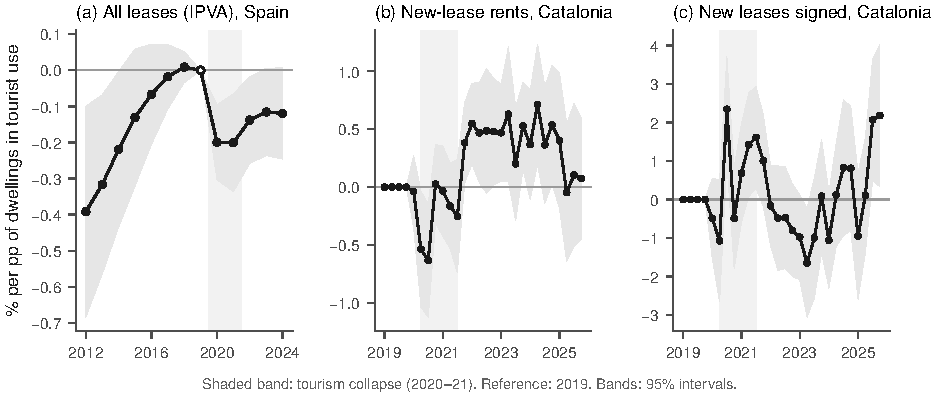
\includegraphics[width=\linewidth]{fig/fig2_tourism.pdf}
\caption{Tourist dwellings and long-term rents around the collapse of tourism}\label{fig:tourism}
\begin{minipage}{0.95\linewidth}\footnotesize\vspace{2pt}
\textit{Notes}: coefficients, multiplied by 100, on the share of dwellings in tourist use in August 2020 interacted with year (a) or quarter (b, c). Panel (a): IPVA, 2012--2024, municipality and province $\times$ year fixed effects, predetermined characteristics $\times$ year, population weights, clusters by province, reference 2019. Panels (b) and (c): Catalan municipalities, municipality and quarter fixed effects, exposure $\times$ calendar quarter, log population $\times$ quarter, population weights, clusters by municipality, reference 2019.
\end{minipage}
\end{figure}

\begin{table}[!htbp]\centering\small
\caption{Tourist dwellings and long-term rents: the 2020--21 collapse of tourism and the recovery}\label{tab:tourism}
\begin{tabular}{lcccc}\toprule
 & \multicolumn{2}{c}{New-lease rents (log)} & \multicolumn{2}{c}{New leases signed (log)}\\\cmidrule(lr){2-3}\cmidrule(lr){4-5}
Exposure (pp of dwellings in tourist use) $\times$ & Coef.$\times$100 & SE & Coef.$\times$100 & SE\\\midrule
2020Q1 (placebo) & $-$0.14 & (0.14) & $-$0.26 & (0.39)\\
Collapse: 2020Q2--2021Q2 & $-$0.30*** & (0.08) & 0.38 & (0.30)\\
Recovery: 2022--2023 & 0.44*** & (0.13) & $-$0.96** & (0.38)\\
2024--2025 & 0.28* & (0.16) & 0.23 & (0.53)\\
Municipalities / observations & \multicolumn{2}{c}{274 / 7480} & \multicolumn{2}{c}{274 / 7671}\\
\bottomrule\end{tabular}
\begin{minipage}{0.92\linewidth}\footnotesize\vspace{4pt}
\textit{Notes}: Catalan municipalities with new leases in every quarter of 2019 and at least 40 in that year; quarters 2019Q1--2025Q4. Exposure: tourist dwellings as a percentage of all dwellings in August 2020 (INE). Regressions include municipality and quarter fixed effects, exposure $\times$ calendar-quarter terms (seasonality of tourist letting) and log 2019 population $\times$ quarter; reference period 2019Q1--2019Q4. Population weights; standard errors clustered by municipality. In 2020 the tourist-stay tax paid by tourist dwellings in Catalonia fell to 21\,\% of its 2019 level and in 2021 it was 60\,\%. *** $p<0.01$, ** $p<0.05$, * $p<0.1$.
\end{minipage}\end{table}

\subsection{Regulation}\label{sec:regulation}

\textit{The cap on updates, 2022--2023.} Under the index identity \eqref{eq:index}, a cap on updates lowers the growth of the index of all leases by $(1-\lambda_t)(\pi_t-u_t)$, whatever happens to market rents. In 2022, existing leases grew by \gExisttwotwo\,\% against consumer price inflation of \cpiYtwotwo\,\%; in 2023, by \gExisttwothree\,\% against \cpiYtwothree\,\%. Had existing leases followed consumer prices, the index of all leases would have been \capGap\,\% higher by 2023 (table~\ref{tab:regulation}, panel C). This is an upper bound, since not all leases are indexed to the CPI; it shows that part of the slow growth of the index of all leases is a direct effect of legislation and not a sign of a calm market.

\textit{The Catalan tensioned-zone cap, 2024--2025.} Prediction P3 states that a binding cap on new contracts lowers their rents and the number of leases signed. The designation was not random: it followed criteria of rent burden and rent growth, and the first wave included the largest municipalities. The paper therefore compares each wave with clean controls: the first wave with municipalities not yet or never designated until the second wave took effect, and each wave with never-designated municipalities to the end of 2025, controlling for tourist exposure and its seasonality \citep{callaway2021,roth2023}. Figure~\ref{fig:cap} shows the event studies. Rents on new leases fell by \capROne\,\% in the first wave relative to not-yet-designated municipalities, by \capROneNever\,\% relative to never-designated municipalities, and by \capRTwo\,\% in the second wave. The number of new leases fell by \capNOne\,\% in the first wave; in the second wave the fall is smaller and not robust. The joint test of pre-period coefficients rejects in the first-wave comparisons: pre-period coefficients fluctuate around zero, in particular in 2021, without a trend, whereas all post-period coefficients for rents are negative. Removing a linear pre-trend estimated on the pre-period leaves the rent estimates between \capRdOne{} and \capRdTwo\,\%. In the sample, the number of new leases signed in Catalonia fell from \catLeasesTwentyThree{} in 2023 to \catLeasesTwentyFive{} in 2025. At the provincial level, the INE index of new leases grew by \provNew{} percentage points less in Catalan provinces in 2024 than elsewhere.

These estimates agree with those of \citet{jofre2023} for the 2020 law and of \citet{perez2026} for the first months of the 2024 cap, and extend them to the end of 2025. The design measures new-lease rents and the number of leases deposited; it cannot say whether the leases not signed became seasonal or room rentals, sales or vacant dwellings, nor whether they moved to the informal market. Fewer deposited leases do not necessarily mean fewer dwellings available to residents.

\begin{figure}[!htbp]\centering
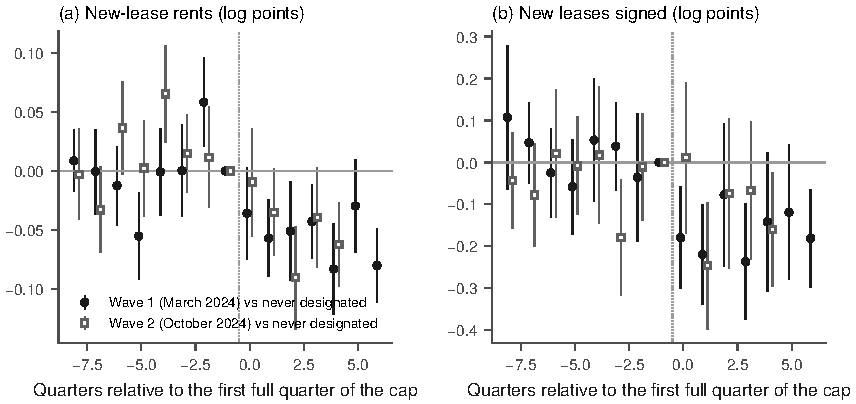
\includegraphics[width=0.95\linewidth]{fig/fig3_cap.pdf}
\caption{Catalan tensioned-zone cap: new-lease rents and leases signed}\label{fig:cap}
\begin{minipage}{0.92\linewidth}\footnotesize\vspace{2pt}
\textit{Notes}: event-study coefficients and 95\,\% intervals, quarters relative to the first full quarter of the cap (2024Q2 for wave 1, 2024Q4 for wave 2), relative to the quarter before. Controls: Catalan municipalities never designated. Municipality and quarter fixed effects, tourist exposure $\times$ calendar quarter and $\times$ period; clusters by municipality.
\end{minipage}
\end{figure}

\begin{table}[!htbp]\centering\small
\caption{Caps on rents: the Catalan tensioned-zone cap (2024) and the cap on annual updates (2022--2023)}\label{tab:regulation}
\begin{adjustbox}{max width=\linewidth}\begin{tabular}{lcccccc}\toprule
 & Treated & Controls & \multicolumn{2}{c}{New-lease rents (log)} & \multicolumn{2}{c}{New leases signed (log)}\\\cmidrule(lr){4-5}\cmidrule(lr){6-7}
 & & & Post & Pre-trend adj. & Post & Pre-trend adj.\\\midrule
\multicolumn{7}{l}{\textit{A. Tensioned-zone cap on new contracts, Catalonia (stacked comparisons, unweighted)}}\\
Wave 1 vs not yet designated, to 2024Q3 & 135 & 139 & $-$0.044 (0.009) & $-$0.037 & $-$0.181 (0.025) & $-$0.187\\
Wave 1 vs never designated, to 2025Q4 & 135 & 36 & $-$0.050 (0.010) & $-$0.052 & $-$0.184 (0.042) & $-$0.160\\
Wave 2 vs never designated, to 2025Q4 & 103 & 36 & $-$0.053 (0.013) & $-$0.067 & $-$0.100 (0.049) & $-$0.052\\
\multicolumn{7}{l}{\textit{Population-weighted}}\\
Wave 1 vs not yet designated, to 2024Q3 & 135 & 139 & $-$0.036 (0.008) & $-$0.037 & $-$0.217 (0.032) & $-$0.208\\
Wave 2 vs never designated, to 2025Q4 & 103 & 36 & $-$0.057 (0.012) & $-$0.076 & $-$0.044 (0.040) & 0.009\\
\addlinespace
\multicolumn{7}{l}{\textit{B. Provinces: growth of the IPVA in 2024, Catalan provinces vs the rest (2022--2024)}}\\
New contracts & 4 & 44 & $-$0.0057 (0.0016) & & & \\
Existing contracts & 4 & 44 & $-$0.0019 (0.0006) & & & \\
\addlinespace
\multicolumn{7}{l}{\textit{C. Cap on annual updates of existing leases (2\,\%), Spain}}\\
2022: growth of existing leases 2.1\,\%, CPI 8.4\,\% & \multicolumn{6}{l}{gap in the index for all leases: 5.2 pp}\\
2023: growth of existing leases 2.4\,\%, CPI 3.5\,\% & \multicolumn{6}{l}{gap in the index for all leases: 1.0 pp}\\
Cumulative 2022--2023 & \multicolumn{6}{l}{index for all leases 6.1\,\% higher if existing leases had followed the CPI}\\
\bottomrule\end{tabular}\end{adjustbox}
\begin{minipage}{0.97\linewidth}\footnotesize\vspace{4pt}
\textit{Notes}: panel A, Catalan municipalities with new leases in every quarter of 2019 (at least 40 in the year); wave 1: 140 municipalities designated on 16 March 2024 (first full quarter 2024Q2); wave 2: 131 designated in October 2024 (first full quarter 2024Q4). Regressions include municipality and quarter fixed effects, tourist-dwelling exposure $\times$ calendar quarter and $\times$ the 2020--21 and 2022--23 periods. Post: average post-treatment coefficient, standard error clustered by municipality in parentheses. Pre-trend adjusted: outcome net of a treated-group linear trend estimated on pre-treatment quarters. Panel B: province and year fixed effects, standard errors clustered by province. Panel C: accounting with INE weights of new and existing leases; it is an upper bound because not all leases are indexed to the CPI and annual averages are used.
\end{minipage}\end{table}

\subsection{Large owners and credit}

\textit{Large owners.} Public data do not identify the owners of rented dwellings by municipality. Two proxies are available. The first is the number of foreclosures on dwellings owned by companies in 2014--2016 per thousand dwellings, a measure of the stock repossessed by banks after the crisis and later sold, often to investment funds; companies accounted for \fjShare\,\% of foreclosures on dwellings in those years. Across 48 provinces, it is not associated with rent growth in 2015--2024 once population growth is controlled for (\fjB{} percentage points per standard deviation, interval \fjLo{} to \fjHi), while population growth is (\provPopB). The second is the share of registered tourist dwellings in Catalonia held by companies, \corpShare\,\% on average. Across municipalities with more than 5,000 inhabitants, it is not associated with the growth of new-lease rents between 2019 and 2025 (\corpB, interval \corpLo{} to \corpHi), whereas the number of tourist dwellings per inhabitant is. Neither result identifies the effect of large owners; together with the small share of companies among landlords documented by \citet{khametshin2024}, they give no support to the view that investment funds drove the rise in rents across municipalities, but they cannot rule out effects in particular neighbourhoods or segments.

\textit{Credit and interest rates.} The 12-month Euribor rose from \eurTwentyOne\,\% in 2021 to \eurTwentyThree\,\% in 2023, and the average rate on new mortgages from \mrTwentyOne\,\% to \mrTwentyThree\,\%. New-lease rents accelerated over the same period, consistent with a shift from buying to renting \citep{khametshin2024}. This is a common shock (P4): with one country and few years, its effect is not identified, and the paper attributes none of the rise to it.

\section{Ranking the determinants}\label{sec:ranking}

Table~\ref{tab:ranking} and figure~\ref{fig:ranking} bring the estimates together for the index of all leases between 2015 and 2024, which grew by \cTotal{} log points. Contributions of different nature are kept apart. Inflation and the cap on updates are accounting contributions, exact under the index identity but not causal. The contributions of local channels are causal within provinces, aggregated under two assumptions that cannot be tested: that there are no spillovers between municipalities and that the national elasticity equals the local one.

\begin{enumerate}
\item \textit{Inflation} accounts for the whole nominal growth of the index of all leases (\cCpi{} log points), through the indexation of existing leases and the nominal rents of new ones.
\item \textit{Legislation on updates} subtracted up to \capGap\,\% (\cCap{} log points) in 2022--2023.
\item \textit{Population growth driven by immigration} is the largest identified local driver: \cPop{} log points (\cPopLo{} to \cPopHi), given an average cumulative inflow of \cPopM\,\% of the population. In the cross-section it accounts for \shPop\,\% of the variance of rent growth within provinces.
\item \textit{Income} is associated with \cInc{} log points (\cIncLo{} to \cIncHi), given mean real income growth of \incReal{} log points in 2015--2023; this contribution is not identified.
\item \textit{Tourist dwellings} contributed \cTourA{} log points in 2015--2019 and \cTourB{} in 2019--2024 at the national level: little on average, because tourist dwellings are a small share of the stock in most municipalities.
\item \textit{Supply} did not respond to demand: the dwelling stock grew by \dlnviv\,\% on average, independently of population inflows. Supply is not a driver of the rise but the reason demand turned into rents.
\item \textit{Rent caps on new contracts} lowered new-lease rents by about 5\,\% in covered Catalan municipalities (\capShare\,\% of the population of the sample), with a negligible effect on the national index so far.
\item \textit{Large owners} and \textit{credit conditions}: no association is found for the former, and the latter are not identified.
\end{enumerate}

\begin{figure}[!htbp]\centering
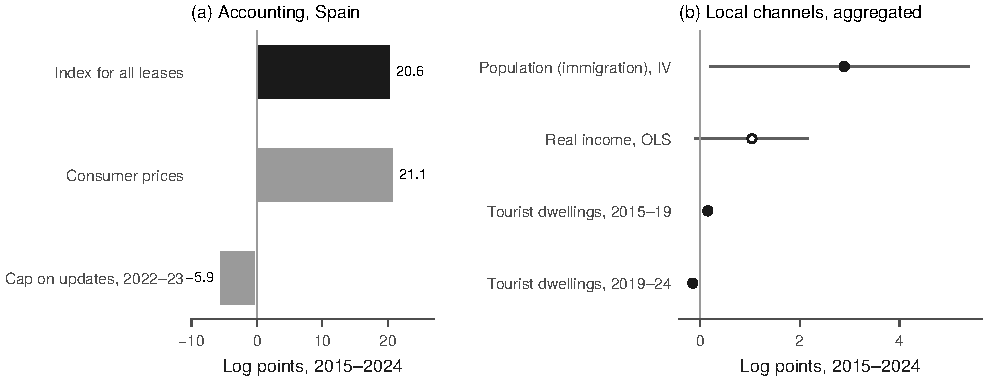
\includegraphics[width=0.98\linewidth]{fig/fig4_ranking.pdf}
\caption{Contributions to the growth of the rent index for all leases, 2015--2024}\label{fig:ranking}
\begin{minipage}{0.95\linewidth}\footnotesize\vspace{2pt}
\textit{Notes}: log points. Panel (a), accounting contributions. Panel (b), local channels aggregated with the mean exposure; horizontal lines are Anderson-Rubin (population) or confidence (income) ranges. Filled markers: identified within provinces; hollow marker: association. See table~\ref{tab:ranking}.
\end{minipage}
\end{figure}

\begin{table}[!htbp]\centering\small
\caption{Contributions to the growth of the rent index for all leases, Spain, 2015--2024 (log points)}\label{tab:ranking}
\begin{adjustbox}{max width=\linewidth}\begin{tabular}{llcll}\toprule
Determinant & Evidence & Contribution & 95\% range & Where it matters\\\midrule
Total growth of the index & & 20.6 & & \\
\addlinespace
General inflation (CPI), via indexation and new contracts & Accounting & 21.1 &  & Common\\
Cap on updates of existing leases, 2022--2023 & Accounting (upper bound) & $-$5.9 &  & Common\\
Population growth driven by immigration & Shift-share IV & 2.9 & [0.2, 5.4] & Larger in big cities\\
Household income (real) & OLS, not identified & 1.0 & [$-$0.1, 2.2] & Uniform\\
Tourist dwellings, 2015--2019 & Event study (exposure) & 0.16 &  & Tourist municipalities\\
Tourist dwellings, 2019--2024 & Event study (exposure) & $-$0.14 &  & Tourist municipalities\\
Supply response of the dwelling stock & Shift-share IV & $\approx$ 0 &  & Absent everywhere\\
Tensioned-zone cap (Catalonia, 2024--) & Stacked DiD (new leases) & -- &  & Catalonia: $-$5.0\,\% on new leases\\
Large owners and investment funds & Not identified & -- &  & No association found\\
Interest rates and credit standards & Not identified & -- &  & Common\\
\bottomrule\end{tabular}\end{adjustbox}
\begin{minipage}{0.97\linewidth}\footnotesize\vspace{4pt}
\textit{Notes}: contributions to the change in the log of the national IPVA between 2015 and 2024. Inflation: change in the log CPI. Update cap: section~\ref{sec:regulation}. Population: within-province long-difference 2SLS elasticity times the population-weighted mean cumulative foreign-born inflow (7.1\,\% of population), range from the Anderson-Rubin set. Income: within-province OLS elasticity times mean real income growth 2015--2023. Tourist dwellings: event-study coefficients times the mean exposure. Aggregation of local elasticities assumes no spillovers across municipalities and a national elasticity equal to the local one; the contributions are not additive and do not sum to the total.
\end{minipage}\end{table}

\textit{By size of municipality.} Figure~\ref{fig:size} applies the common elasticities to the exposure of each size class. The largest cities combine the highest rent growth (\szER{} log points) with the largest foreign-born inflows (\szEInfl\,\% of the population, an implied contribution of \szEPop{} log points against \szAPop{} in municipalities of 10,000--20,000 inhabitants), while the dwelling stock grew at a similar rate, about 4\,\%, in every size class. Tourist dwellings are, on average, a larger share of the stock in small and medium municipalities (\szAVut\,\% and \szBVut\,\% in 2020) than in cities of 100,000--500,000 inhabitants (\szDVut\,\%), and the tail matters: in the 10\,\% most touristic municipalities of 10,000--50,000 inhabitants, \szAVutNinety\,\% or more of dwellings were in tourist use, and in the top 5\,\% of the sample at least 8\,\% (up to 23\,\%). Applying the estimates of section~\ref{sec:determinants}, in a municipality with 13\,\% of dwellings in tourist use the tourism channel moves new-lease rents by 4--6\,\%, of the same order as the population channel; at the median exposure (0.3\,\%) it is negligible. In the large cities, population dominates. The tensioned-zone cap applies mainly to large and medium Catalan municipalities.

\begin{figure}[!htbp]\centering
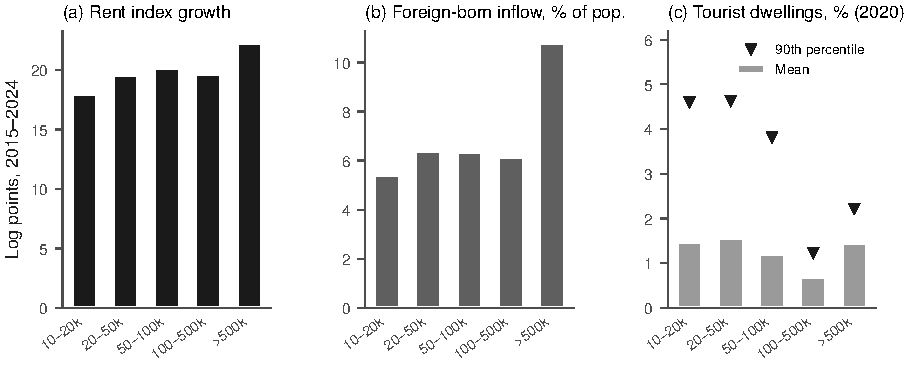
\includegraphics[width=\linewidth]{fig/fig5_size.pdf}
\caption{Rent growth and exposure to each channel by size of municipality}\label{fig:size}
\begin{minipage}{0.95\linewidth}\footnotesize\vspace{2pt}
\textit{Notes}: IPVA municipalities by 2015 population. (a) Growth of the log index of all leases, 2015--2024. (b) Cumulative foreign-born net inflow, 2016--2024. (c) Share of dwellings in tourist use, August 2020: mean and 90th percentile. Means weighted by population.
\end{minipage}
\end{figure}

\section{Discussion}\label{sec:discussion}

\textit{What the evidence supports.} The rise in rents that drives the public debate is a rise in new-lease rents in large cities and tourist areas, not in the average rent paid by Spanish tenants. Most of it is common to municipalities within provinces. Among local factors, immigration-driven population growth against an unresponsive housing stock is the most important identified driver. Tourist dwellings displace residents where they are common, and the effect is reversible. Caps on rents lower measured rents, and the cap on new contracts also reduces the number of leases signed.

\textit{What is compatible but not demonstrated.} The common component may reflect national population growth, the user cost of owning, credit standards, construction costs and the expectations of landlords; none of them is identified here. The faster growth of new-lease rents may partly be a response of landlords to longer leases and capped updates, which make the first rent of a lease more important; the falling share of new leases in the index is consistent with lower mobility of tenants, but the paper does not test either mechanism. Income growth is associated with rent growth, but the direction of causality is not established.

\textit{What is not supported.} The data give no support to the view that investment funds or large owners drove the rise across municipalities, and no support to the view that the stock of dwellings expanded in response to demand. The absence of a statistically significant association is not evidence of no effect: the intervals for large owners are wide and the proxies are coarse.

\textit{Prices are not welfare.} Higher rents transfer income from tenants to landlords and lower the welfare of tenants who pay them, but they also reflect the value of locations and the absorption of population. The companion paper shows that much of the population growth was housed through higher occupancy of existing dwellings; higher occupancy is not the same as overcrowding, and neither paper measures the welfare of the households concerned. Caps lower measured rents for those who sign a lease but reduce the number of leases; their net effect on welfare depends on who obtains and who loses access, which the data do not show.

\textit{Limitations.} The index of all leases excludes the Basque Country, Navarre and municipalities with fewer than 10,000 inhabitants. New-lease rents are observed only in Catalonia. Tourist-dwelling counts start in August 2020, during the shock used for identification, so exposure is measured in the first months of the collapse; listings that disappeared before August 2020 are not counted, which would bias the exposure measure towards zero in the most affected places. The aggregation of local elasticities to the national level assumes away spillovers and general-equilibrium effects. Ownership data by municipality would be needed to study large owners, and comparable new-lease data for all regions to study rent caps and tourism outside Catalonia; the Ministry of Housing's rent reference system (SERPAVI) and the deposit registers of other regions are natural candidates if they become accessible.

\section{Conclusion}\label{sec:conclusion}

Spanish rents rose because demand grew in places where the housing stock did not respond, and because tourist letting removed dwellings from residents where it was common; inflation and the indexation of leases account for the nominal growth of the average rent, while caps held it down. The policy implications follow from the ranking. Measures that expand the supply of dwellings available to residents in large cities address the main identified local driver; restrictions on tourist dwellings matter in tourist municipalities; caps lower measured rents at the cost of fewer leases. Monitoring the market requires new-lease data for all regions: an index of all leases moves too slowly, and is too affected by legislation, to describe what new tenants face.

\section*{Declarations}
\noindent\textbf{Funding} No funding was received for this work.\\
\textbf{Competing interests} The author declares no competing interests.\\
\textbf{Data and code availability} All data are public and are downloaded by the replication code from INE, the Generalitat de Catalunya, the ECB and the companion paper's replication package; the code is available from the author.\\
\textbf{Use of generative AI} Claude (Anthropic) was used to retrieve the data and to assist with the code, the drafting and the English translation. The author verified all results and text and is fully responsible for the article.

\begin{thebibliography}{99}\small\setlength{\itemsep}{1pt}
\bibitem[Adão et~al.(2019)]{adao2019} Adão R, Kolesár M, Morales E (2019) Shift-share designs: theory and inference. The Quarterly Journal of Economics 134(4):1949--2010. \url{https://doi.org/10.1093/qje/qjz025}
\bibitem[Almagro and Domínguez-Iino(2025)]{almagro2025} Almagro M, Domínguez-Iino T (2025) Location sorting and endogenous amenities: evidence from Amsterdam. Econometrica 93(3):1031--1071. \url{https://doi.org/10.3982/ECTA21394}
\bibitem[Ambrose et~al.(2015)]{ambrose2015} Ambrose BW, Coulson NE, Yoshida J (2015) The repeat rent index. The Review of Economics and Statistics 97(5):939--950. \url{https://doi.org/10.1162/REST_a_00500}
\bibitem[Autor et~al.(2014)]{autor2014} Autor DH, Palmer CJ, Pathak PA (2014) Housing market spillovers: evidence from the end of rent control in Cambridge, Massachusetts. Journal of Political Economy 122(3):661--717. \url{https://doi.org/10.1086/675536}
\bibitem[Barron et~al.(2021)]{barron2021} Barron K, Kung E, Proserpio D (2021) The effect of home-sharing on house prices and rents: evidence from Airbnb. Marketing Science 40(1):23--47. \url{https://doi.org/10.1287/mksc.2020.1227}
\bibitem[Batalha et~al.(2022)]{batalha2022} Batalha M, Gonçalves D, Peralta S, Pereira dos Santos J (2022) The virus that devastated tourism: the impact of covid-19 on the housing market. Regional Science and Urban Economics 95:103774. \url{https://doi.org/10.1016/j.regsciurbeco.2022.103774}
\bibitem[Borusyak et~al.(2022)]{borusyak2022} Borusyak K, Hull P, Jaravel X (2022) Quasi-experimental shift-share research designs. The Review of Economic Studies 89(1):181--213. \url{https://doi.org/10.1093/restud/rdab030}
\bibitem[Callaway and Sant'Anna(2021)]{callaway2021} Callaway B, Sant'Anna PHC (2021) Difference-in-differences with multiple time periods. Journal of Econometrics 225(2):200--230. \url{https://doi.org/10.1016/j.jeconom.2020.12.001}
\bibitem[Chaves-Fonseca(2026)]{chaves2026} Chaves-Fonseca C (2026) The effect of short-term rentals on house prices and residential mobility: evidence from Madrid. SERIEs. \url{https://doi.org/10.1007/s13209-026-00335-2}
\bibitem[Cocola-Gant et~al.(2025)]{cocola2025} Cocola-Gant A, Hodkinson SN, Janoschka M (2025) The financialisation of short-term rentals in Barcelona: property ownership and the consolidation of a new asset class. European Urban and Regional Studies 33(3):300--317. \url{https://doi.org/10.1177/09697764251361724}
\bibitem[Diamond et~al.(2019)]{diamond2019} Diamond R, McQuade T, Qian F (2019) The effects of rent control expansion on tenants, landlords, and inequality: evidence from San Francisco. American Economic Review 109(9):3365--3394. \url{https://doi.org/10.1257/aer.20181289}
\bibitem[DiPasquale and Wheaton(1992)]{dipasquale1992} DiPasquale D, Wheaton WC (1992) The markets for real estate assets and space: a conceptual framework. Real Estate Economics 20(2):181--198. \url{https://doi.org/10.1111/1540-6229.00579}
\bibitem[Duso et~al.(2024)]{duso2024} Duso T, Michelsen C, Schäfer M, Tran KD (2024) Airbnb and rental markets: evidence from Berlin. Regional Science and Urban Economics 106:104007. \url{https://doi.org/10.1016/j.regsciurbeco.2024.104007}
\bibitem[Fernández-Aguilera(2026)]{fernandez2026} Fernández-Aguilera VM (2026) Absorbed by crowding: immigration, rents and housing occupancy in Spain. Unpublished manuscript, University of Almería
\bibitem[Franco and Santos(2021)]{franco2021} Franco SF, Santos CD (2021) The impact of Airbnb on residential property values and rents: evidence from Portugal. Regional Science and Urban Economics 88:103667. \url{https://doi.org/10.1016/j.regsciurbeco.2021.103667}
\bibitem[Garcia-López et~al.(2020)]{garcialopez2020} Garcia-López M-À, Jofre-Monseny J, Martínez-Mazza R, Segú M (2020) Do short-term rental platforms affect housing markets? Evidence from Airbnb in Barcelona. Journal of Urban Economics 119:103278. \url{https://doi.org/10.1016/j.jue.2020.103278}
\bibitem[Garriga et~al.(2023)]{garriga2023} Garriga C, Gete P, Tsouderou A (2023) The economic effects of real estate investors. Real Estate Economics 51(3):655--685. \url{https://doi.org/10.1111/1540-6229.12427}
\bibitem[Genesove(2003)]{genesove2003} Genesove D (2003) The nominal rigidity of apartment rents. The Review of Economics and Statistics 85(4):844--853. \url{https://doi.org/10.1162/003465303772815763}
\bibitem[Glaeser and Gyourko(2005)]{glaeser2005} Glaeser EL, Gyourko J (2005) Urban decline and durable housing. Journal of Political Economy 113(2):345--375. \url{https://doi.org/10.1086/427465}
\bibitem[Glaeser and Gyourko(2018)]{glaeser2018} Glaeser E, Gyourko J (2018) The economic implications of housing supply. Journal of Economic Perspectives 32(1):3--30. \url{https://doi.org/10.1257/jep.32.1.3}
\bibitem[Goldsmith-Pinkham et~al.(2020)]{goldsmith2020} Goldsmith-Pinkham P, Sorkin I, Swift H (2020) Bartik instruments: what, when, why, and how. American Economic Review 110(8):2586--2624. \url{https://doi.org/10.1257/aer.20181047}
\bibitem[Gonzalez and Ortega(2013)]{gonzalez2013} Gonzalez L, Ortega F (2013) Immigration and housing booms: evidence from Spain. Journal of Regional Science 53(1):37--59. \url{https://doi.org/10.1111/jors.12010}
\bibitem[Gurun et~al.(2023)]{gurun2023} Gurun UG, Wu J, Xiao SC, Xiao SW (2023) Do Wall Street landlords undermine renters' welfare? The Review of Financial Studies 36(1):70--121. \url{https://doi.org/10.1093/rfs/hhac017}
\bibitem[Gyourko et~al.(2013)]{gyourko2013} Gyourko J, Mayer C, Sinai T (2013) Superstar cities. American Economic Journal: Economic Policy 5(4):167--199. \url{https://doi.org/10.1257/pol.5.4.167}
\bibitem[Hilber and Vermeulen(2016)]{hilber2016} Hilber CAL, Vermeulen W (2016) The impact of supply constraints on house prices in England. The Economic Journal 126(591):358--405. \url{https://doi.org/10.1111/ecoj.12213}
\bibitem[Himmelberg et~al.(2005)]{himmelberg2005} Himmelberg C, Mayer C, Sinai T (2005) Assessing high house prices: bubbles, fundamentals and misperceptions. Journal of Economic Perspectives 19(4):67--92. \url{https://doi.org/10.1257/089533005775196769}
\bibitem[Hsieh and Moretti(2019)]{hsieh2019} Hsieh C-T, Moretti E (2019) Housing constraints and spatial misallocation. American Economic Journal: Macroeconomics 11(2):1--39. \url{https://doi.org/10.1257/mac.20170388}
\bibitem[Janoschka et~al.(2020)]{janoschka2020} Janoschka M, Alexandri G, Ramos HO, Vives-Miró S (2020) Tracing the socio-spatial logics of transnational landlords' real estate investment: Blackstone in Madrid. European Urban and Regional Studies 27(2):125--141. \url{https://doi.org/10.1177/0969776418822061}
\bibitem[Jofre-Monseny et~al.(2023)]{jofre2023} Jofre-Monseny J, Martínez-Mazza R, Segú M (2023) Effectiveness and supply effects of high-coverage rent control policies. Regional Science and Urban Economics 101:103916. \url{https://doi.org/10.1016/j.regsciurbeco.2023.103916}
\bibitem[Khametshin et~al.(2024)]{khametshin2024} Khametshin D, López Rodríguez D, Pérez García L (2024) El mercado del alquiler de vivienda residencial en España: evolución reciente, determinantes e indicadores de esfuerzo. Documentos Ocasionales 2432, Banco de España, Madrid. \url{https://doi.org/10.53479/37872}
\bibitem[Kholodilin(2024)]{kholodilin2024} Kholodilin KA (2024) Rent control effects through the lens of empirical research: an almost complete review of the literature. Journal of Housing Economics 63:101983. \url{https://doi.org/10.1016/j.jhe.2024.101983}
\bibitem[Koster et~al.(2021)]{koster2021} Koster HRA, van Ommeren J, Volkhausen N (2021) Short-term rentals and the housing market: quasi-experimental evidence from Airbnb in Los Angeles. Journal of Urban Economics 124:103356. \url{https://doi.org/10.1016/j.jue.2021.103356}
\bibitem[Mills et~al.(2019)]{mills2019} Mills J, Molloy R, Zarutskie R (2019) Large-scale buy-to-rent investors in the single-family housing market: the emergence of a new asset class. Real Estate Economics 47(2):399--430. \url{https://doi.org/10.1111/1540-6229.12189}
\bibitem[Molloy(2020)]{molloy2020} Molloy R (2020) The effect of housing supply regulation on housing affordability: a review. Regional Science and Urban Economics 80:103350. \url{https://doi.org/10.1016/j.regsciurbeco.2018.03.007}
\bibitem[Monràs and Garcia-Montalvo(2023)]{monras2023} Monràs J, Garcia-Montalvo J (2023) The effect of second-generation rent controls: new evidence from Catalonia. Working Paper 2023-28, Federal Reserve Bank of San Francisco. \url{https://doi.org/10.24148/wp2023-28}
\bibitem[Pérez García(2026)]{perez2026} Pérez García L (2026) Effectiveness of rent controls: evidence from Spain. arXiv preprint 2602.08631
\bibitem[Poterba(1984)]{poterba1984} Poterba JM (1984) Tax subsidies to owner-occupied housing: an asset-market approach. The Quarterly Journal of Economics 99(4):729--752. \url{https://doi.org/10.2307/1883123}
\bibitem[Roback(1982)]{roback1982} Roback J (1982) Wages, rents, and the quality of life. Journal of Political Economy 90(6):1257--1278. \url{https://doi.org/10.1086/261120}
\bibitem[Roth et~al.(2023)]{roth2023} Roth J, Sant'Anna PHC, Bilinski A, Poe J (2023) What's trending in difference-in-differences? A synthesis of the recent econometrics literature. Journal of Econometrics 235(2):2218--2244. \url{https://doi.org/10.1016/j.jeconom.2023.03.008}
\bibitem[Sá(2015)]{sa2015} Sá F (2015) Immigration and house prices in the UK. The Economic Journal 125(587):1393--1424. \url{https://doi.org/10.1111/ecoj.12158}
\bibitem[Saiz(2007)]{saiz2007} Saiz A (2007) Immigration and housing rents in American cities. Journal of Urban Economics 61(2):345--371. \url{https://doi.org/10.1016/j.jue.2006.07.004}
\bibitem[Saiz(2010)]{saiz2010} Saiz A (2010) The geographic determinants of housing supply. The Quarterly Journal of Economics 125(3):1253--1296. \url{https://doi.org/10.1162/qjec.2010.125.3.1253}
\bibitem[Sanchis-Guarner(2023)]{sanchis2023} Sanchis-Guarner R (2023) Decomposing the impact of immigration on house prices. Regional Science and Urban Economics 100:103893. \url{https://doi.org/10.1016/j.regsciurbeco.2023.103893}
\bibitem[Sinai and Souleles(2005)]{sinai2005} Sinai T, Souleles NS (2005) Owner-occupied housing as a hedge against rent risk. The Quarterly Journal of Economics 120(2):763--789. \url{https://doi.org/10.1093/qje/120.2.763}
\bibitem[Valentin(2021)]{valentin2021} Valentin M (2021) Regulating short-term rental housing: evidence from New Orleans. Real Estate Economics 49(1):152--186. \url{https://doi.org/10.1111/1540-6229.12330}
\end{thebibliography}


\end{document}
